\documentclass[12pt,a4paper]{report}
\usepackage[utf8]{inputenc}
\usepackage[T1]{fontenc}
\usepackage[french]{babel}
\usepackage{graphicx}
\usepackage{geometry}
\usepackage{setspace}
\usepackage{hyperref}
\usepackage{titlesec}
\usepackage{xcolor}
\geometry{margin=2.5cm}
\usepackage{array}   % Pour personnaliser les colonnes
\usepackage[none]{hyphenat} % dans le préambule
\usepackage{float}
\usepackage{makecell}


\onehalfspacing

\titleformat{\chapter}[display]
{\normalfont\bfseries\huge}{\chaptername\ \thechapter}{20pt}{\Huge}
\titleformat{\section}
{\normalfont\Large\bfseries}{\thesection}{1em}{}

\begin{document}
	
	\tableofcontents
	
	\chapter{Contexte du Projet}
	
	\section{Projet de Fin d’Études}
	
	Ce projet s’inscrit dans le cadre de la validation de mon cursus de fin d’études en Génie Informatique à l'Ecole des Hautes Etudes d'Ingénierie , et a été réalisé au sein de l’entreprise Algolus, située à Oujda. Le stage a débuté le 3 Mars 2024, avec pour objectif principal la conception et le développement d’une application intelligente de détection et de correction d’erreurs logicielles basée sur une approche RAG multimodale.
	
	Ce stage a constitué une excellente opportunité de mettre en pratique les connaissances acquises durant ma formation, tout en découvrant les réalités professionnelles du développement logiciel orienté intelligence artificielle.
	
	\section{Entreprise d’accueil}
	
	\begin{figure}[H]
		\centering
		
\includegraphics[width=0.3\textwidth]{algolus-logo.png}
		\caption{Logo de Algolus}
		\label{fig:algolus-logo}
	\end{figure}
	
	\subsection{Description de l’entreprise}
	
	Algolus est une agence web marocaine, créée en 2020, spécialisée dans la conception et le développement de solutions informatiques adaptées aux besoins des clients. Elle s'engage à offrir à ses clients une communication en ligne efficace et sur mesure.

	Ses prestations incluent :
	
	\begin{itemize}
		\item Création et gestion de sites web (dynamiques, statiques, e-commerce, CMS)
		\item Développement d'applications web (mode hybride)
		\item Stratégie digitale complète :
		\begin{itemize}
			\item[•] Infographie			
			\item[•] Publicité en ligne			
			\item[•] Marketing digital			
			\item[•] Community management			
			\item[•] E-réputation			
		\end{itemize}
	\end{itemize}
	
	\subsection{Fiche technique de l'entreprise}
	
	Le tableau ci-dessous récapitule la fiche technique de l'entreprise Algolus :
	
	\begin{table}[htbp]
		\centering
		\caption{Fiche technique de l'entreprise Algolus}  % Le titre apparaît au-dessus
		\begin{tabular}{|l|l|}
			\hline
			\textbf{Dénomination sociale} & Algolus \\
			\hline
			\textbf{Date de création} & 07/10/2020 \\
			\hline
			\textbf{Forme juridique} & SARL \\
			\hline
			\textbf{Capital} & 100.000 Dh \\
			\hline
			\textbf{Chiffre d'affaires} & Indisponible \\
			\hline
			\textbf{Activités} & Développement informatique et marketing digital \\
			\hline
			\textbf{Effectif} & 10 \\
			\hline
			\textbf{Dirigeant} & Radwane BERAHIOUI \\
			\hline
			\textbf{Coordonnées} & \makecell[l]{+212 6644 35967 \\ Redwan.Berahioui@algolus.ma \\ www.algolus.ma \\ IMMEUBLE OUASSIM, Bd Mohammed VI, Oujda 60000} \\
			\hline
		\end{tabular}
		\label{tab:fiche-technique-algolus}  % Pour référence avec \ref
	\end{table}
	
	\subsection{Organigramme de l’entreprise}
	
	La figure ci-dessous présente l'organigramme de l'entreprise Algolus :
	
	\begin{figure}[H]
		\centering
		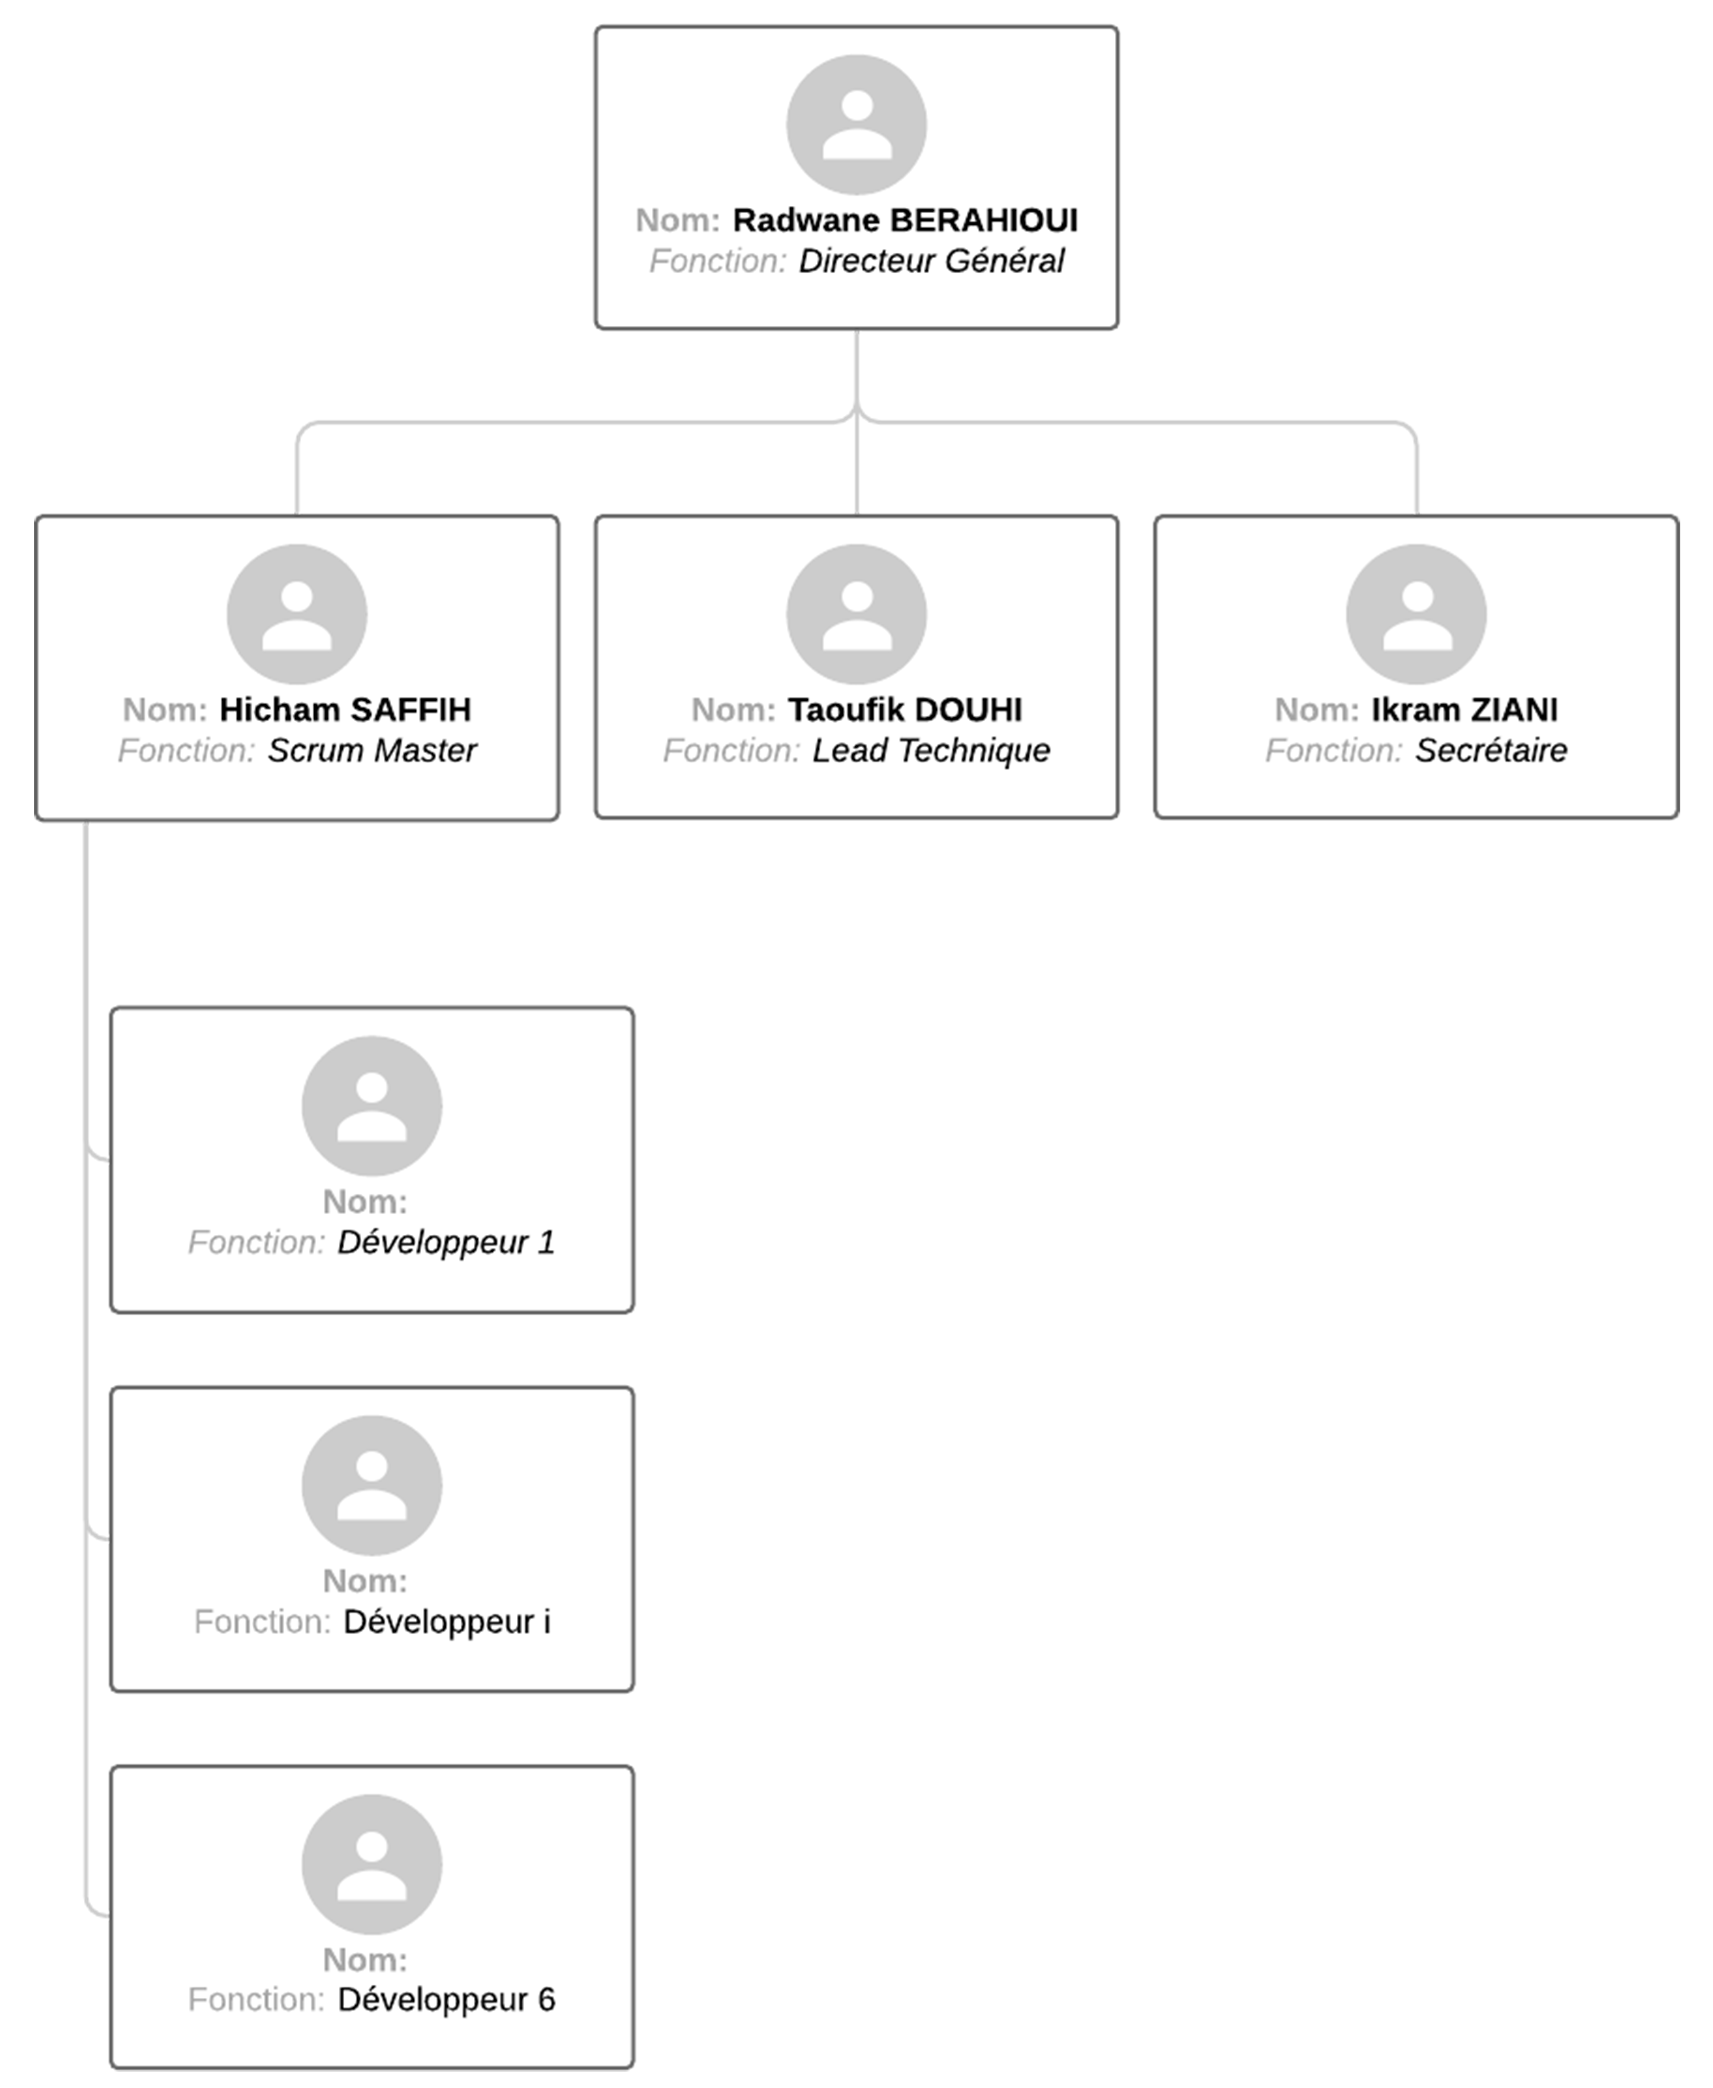
\includegraphics[width=1\textwidth]{algolus-organigramme.png}
		\caption{Organigramme de l'entreprise Algolus}
		\label{fig:algolus-organigramme}
	\end{figure}
	
	\section{Description des besoins}
	
	\subsection{Problématique}
	
	Dans le développement logiciel, la détection et la correction des erreurs représentent un défi majeur, notamment en raison de la diversité des sources d’anomalies (logs, stack traces, captures d’écran, retours utilisateurs, etc.) et de la complexité croissante des applications. Les méthodes traditionnelles de débogage reposent souvent sur une analyse manuelle, ce qui est chronophage et sujet à des erreurs humaines. De plus, les solutions existantes peinent à offrir une approche unifiée et intelligente pour interpréter ces anomalies et proposer des correctifs pertinents.
	
	L’absence d’un système capable de :
	
	\begin{itemize}
		\item Comprendre multimodalement les erreurs (texte, images, logs structurés).
		
		\item Proposer des corrections automatisées en s’appuyant sur des modèles de langage (LLMs) et des techniques de RAG (Retrieval-Augmented Generation).
		
		\item S’intégrer facilement dans des environnements DevOps existants.
	\end{itemize}
	
	rend ce projet particulièrement pertinent. Comment concevoir une application IA capable d’analyser efficacement ces différentes sources d’erreurs et de générer des solutions adaptées et contextualisées ?
	
	\subsection{Solutions envisagées}
	
	Pour répondre à cette problématique, le projet s’appuie sur une architecture innovante :
	
	\begin{enumerate}
		\item Analyse Multimodale des Erreurs :
		\begin{itemize}
			\item Implémenter un système capable d’interpréter des données hétérogènes (stack traces, logs texte, captures d’écran, etc.).
			\item Utiliser des techniques de RAG pour enrichir les requêtes avec une base de connaissances (documentation technique, résolutions d’erreurs courantes).
		\end{itemize}
		
		\item Génération Automatique de Correctifs :
		\begin{itemize}
			\item Exploiter des LLMs (via Ollama) pour suggérer des corrections précises et contextualisées.
		\end{itemize}
		
		\item Intégration et Scalabilité :
		\begin{itemize}
			\item Développer un backend Spring Boot flexible, couplé à LangChain4J pour orchestrer les appels IA, et un système de gestion de base de données qui prend en charge les bases de données vectorielles, comme PostgeSQL.
			
			\item Permettre une extension future via des connecteurs pour différents outils de monitoring.
		\end{itemize}
		
		\item Optimisation et Évaluation :
		\begin{itemize}
			\item Mesurer l’efficacité du système via des métriques de précision (taux de détection, pertinence des correctifs).
			
			\item Benchmark : Comparaison sur des jeux de données communs.
		\end{itemize}
	\end{enumerate}
	
	\subsection{Objectifs}
	
	Ce projet vise à développer une application intelligente et modulaire permettant de détecter et de corriger automatiquement les anomalies logicielles. Les objectifs spécifiques incluent :
	
	\begin{itemize}
		\item Détecter avec un bon taux de réussite les anomalies logicielles sur des sources multimodales.
		
		\item Proposer des correctifs pertinents dans la majorités des cas.
		
		\item Optimiser le temps moyen de résolution d’erreurs par rapport aux méthodes manuelles.
	\end{itemize}
	
	\subsection{Les besoins fonctionnels}
	
	\begin{enumerate}
		
		\item Collecte et Pré-traitement des Données
		
		Extraction automatique des erreurs à partir de :
		\begin{itemize}
			\item Stacktraces : Parsing des logs pour identifier les exceptions (ex: NullPointerException).			
			\item Captures d’écran : Utilisation de modèles de vision par IA pour détecter les messages d’erreur visuels.
			\item Retours utilisateurs : Analyse NLP des descriptions textuelles (ex: "Le bouton ne répond pas").
		\end{itemize}
		
		\item Analyse et Compréhension
		\begin{itemize}
			\item Analyse sémantique des messages d’erreur.
			\item Enrichissement contextuel : requêtage d’une base de connaissances (documentation technique, correctifs historiques) via RAG.
		\end{itemize}
		
		\item Génération de Solutions
		\begin{itemize}
			\item Explication en langage naturel des causes racines.
			\item Génération de correctifs par Ollama (ex: snippets de code, étapes de résolution).
		\end{itemize}
		
		\item Interfaces utilisateurs
		\begin{itemize}
			\item Soumission des erreurs : Formulaires web pour uploader des stacktraces et des captures d'écran
			\item Visualisation des résultats : Dashboard interactif (erreurs en cours, historiques, statistiques).
		\end{itemize}
		
	\end{enumerate}
	
	\subsection{Les besoins non fonctionnels}
	
	Les besoins non fonctionnels spécifient comment le système doit fonctionner, sans décrire des fonctionnalités précises. Ils couvrent des aspects comme les performances, la sécurité, ou l’ergonomie.
	
	Les besoins non fonctionnels définies dans notre système sont :
	
	\begin{enumerate}
		
		\item Performances
		
		\begin{itemize}
			\item Temps de réponse optimisé.	
			\item Scalabilité : Support de plusieurs requêtes simultanées.
		\end{itemize}
		
		\item Intégration et Interopérabilité
		\begin{itemize}
			\item API REST : Endpoints standardisés et format de réponse avec schéma cohérent.
			\item Support offline : Fonctionnement local avec Ollama.
		\end{itemize}
		
		\item Sécurité et Confidentialité
		\begin{itemize}
			\item Protection des données : chiffrement des échanges et anonymisation des logs utilisateurs (RGPD).
			\item Authentification : JWT pour l’accès aux APIs sensibles.
		\end{itemize}
		
		\item Expérience Utilisateur
		
		Ergonomie : interface intuitive, Dark/Light mode et thèmes accessibles.
		\begin{itemize}
			\item Soumission des erreurs : Formulaires web pour uploader des stacktraces et des captures d'écran
			\item Visualisation des résultats : Dashboard interactif (erreurs en cours, historiques, statistiques).
		\end{itemize}
		
	\end{enumerate}
	
	\chapter{Analyse et modélisation}
	
	\section{Importance de l'analyse}
	
	L’analyse constitue une étape clé dans tout projet de développement informatique, car elle permet de bien comprendre les besoins du client et les contraintes du système à réaliser. Elle sert à identifier les fonctionnalités attendues, à détecter les éventuelles incohérences et à poser les bases d’une conception solide. Une analyse bien menée réduit considérablement les risques d’erreurs en phase de développement, facilite la planification du travail et améliore la qualité globale du produit final. Elle est donc essentielle pour assurer la réussite du projet.	
	
	\section{Unified Modeling Language}
	
	Dans le cadre d’un projet de développement informatique, la modélisation UML (Unified Modeling Language) joue un rôle essentiel en facilitant la compréhension, la conception et la communication autour du système à développer. UML propose un ensemble normalisé de diagrammes qui permettent de représenter visuellement les différentes dimensions d’un logiciel, telles que la structure, le comportement et les interactions entre les composants.
	
	L’utilisation de diagrammes UML, comme les diagrammes de cas d’utilisation, de classes ou de séquence, permet de :
	
	\begin{itemize}
		\item Clarifier les besoins fonctionnels et non fonctionnels dès les premières phases du projet,		
		\item Favoriser une meilleure communication entre les développeurs, les analystes et les clients,		
		\item Détecter plus tôt les incohérences ou erreurs potentielles dans la conception,		
		\item Servir de documentation technique structurée pour le développement, les tests et la maintenance future du logiciel.
	\end{itemize}
	
	Ainsi, UML constitue un outil précieux pour assurer la qualité, la cohérence et la pérennité d’un projet informatique, en apportant une vision globale et partagée du système.
	
	\section{Diagramme de cas d'utilisation}
	
	\subsection{Définition}
	
	Un diagramme de cas d'utilisation est une représentation visuelle des interactions entre les acteurs (utilisateurs, systèmes) et les fonctionnalités d'une application. Il identifie les besoins métiers sous forme d'actions (cas d’utilisation) et montre qui fait quoi, sans entrer dans les détails techniques.
	
	\subsection{Acteurs}
	
	Dans un diagramme de cas d'utilisation, les acteurs sont les entités qui interagissent avec le système pour accomplir un objectif précis. Un acteur peut être primaire (s'il est déclencheur d'un cas d'utilisation) ou secondaire (intervient dans un cas d'utilisation mais ne le déclenche pas). D'une autre part, un acteur peut être humain ou bien un acteur système.
	
	Trois types d'acteurs sont impliqués dans notre cas :
	
	\begin{itemize}
		\item \textbf{Utilisateur} : peut être un développeur ou un testeur qui rapporte une erreur, et peut interagir via une API REST ou bien une interface web.
		
		\item \textbf{Administrateur du système} : responsable de la mise à jour des connaissances du système et de la configuration des modèles.
		
		\item \textbf{Système} : le moteur de traitement intelligent, responsable d'analyser les anomalies, et de proposer des correctifs appropriés.
	\end{itemize}
	
	\subsection{Notre diagramme de cas d'utilisation}
	
	La figure ci-dessous présente le diagramme de cas d'utilisation de notre application :
	
	\begin{figure}[H]
		\centering
		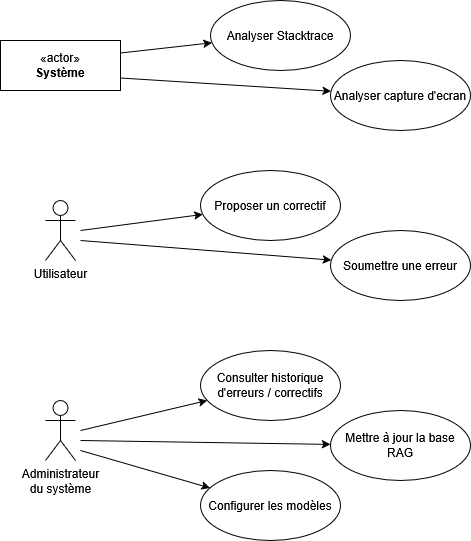
\includegraphics{use-case.drawio.png}
		\caption{Diagramme de cas d'utilisation}
		\label{fig:use-case}
	\end{figure}	
	
	\chapter{Réalisation}

	\section{Stack technique}
	
	\subsection{Langages}
	
	\subsubsection{Java}
	
	\begin{figure}[H]
		\begin{minipage}{0.8\textwidth}
			Java est un langage de programmation orienté objet, robuste et multiplateforme, largement utilisé dans le développement d'applications d'entreprise. Sa forte typographie, sa gestion automatique de la mémoire (via le garbage collector) et son écosystème riche (bibliothèques, frameworks) en font un choix idéal pour les systèmes backend complexes.
		\end{minipage}
		\hfill
		\begin{minipage}{0.15\textwidth}
			\begin{figure}[H]
				\centering
				
\includegraphics[width=\linewidth]{java-logo.png}
				\label{fig:java-logo}
			\end{figure}			
		\end{minipage}
	\end{figure}
		
	\subsection{Frameworks}
	
	\subsubsection{Spring}
	
	\begin{figure}[H]
		\begin{minipage}{0.8\textwidth}
			Spring est un framework modulaire pour Java, simplifiant le développement d'applications grâce à l’inversion de contrôle (IoC) et la programmation orientée aspect (AOP).
		\end{minipage}
		\hfill
		\begin{minipage}{0.15\textwidth} 
			\begin{figure}[H]
				\centering
				
\includegraphics[width=\linewidth]{spring-logo.png}
				\label{fig:spring-logo}
			\end{figure}
		\end{minipage}
	\end{figure}
	
	\subsubsection{Spring Boot}
	
	\begin{figure}[H]
		\begin{minipage}{0.8\textwidth}
			Spring Boot étend Spring en fournissant des configurations automatiques, un serveur embarqué (Tomcat, Netty) et des outils clés en main (Spring Data, Spring Security), permettant de créer des applications standalone rapidement.
		\end{minipage}
		\hfill
		\begin{minipage}{0.15\textwidth} 
			\begin{figure}[H]
				\centering
				
\includegraphics[width=\linewidth]{spring-boot-logo.png}
				\label{fig:spring-boot-logo}
			\end{figure}
		\end{minipage}
	\end{figure}
	
	
	\subsubsection{LangChain4j}
	
	\begin{figure}[H]
		\begin{minipage}{0.8\textwidth}
				LangChain4J est une bibliothèque Java inspirée de LangChain (Python), conçue pour intégrer facilement des LLMs (Modèles de Langage) dans des applications. Elle offre des abstractions pour la gestion des prompts, le RAG, les appels aux modèles (OpenAI, Ollama, etc.), et la connexion à des bases de données vectorielles.
		\end{minipage}
		\hfill
		\begin{minipage}{0.15\textwidth} 
			\begin{figure}[H]
				\centering
				
\includegraphics[width=\linewidth]{langchain4j-logo.png}
				\label{fig:langchain4j-logo}
			\end{figure}
		\end{minipage}
	\end{figure}
	
	\subsection{Bibliothèques}
	
	\subsubsection{Apache Commons}
	
	\begin{figure}[H]
		\begin{minipage}{0.8\textwidth}
			Apache Commons est une bibliothèque Java open-source fournissant des composants réutilisables pour simplifier le développement. Dans ce projet, elle sert à combler des besoins techniques récurrents avec des solutions optimisées et robustes.
		\end{minipage}
		\hfill
		\begin{minipage}{0.15\textwidth} 
			\begin{figure}[H]
				\centering
				
\includegraphics[width=\linewidth]{apache-commons-logo.png}
				\label{fig:apache-commons-logo}
			\end{figure}
		\end{minipage}
	\end{figure}
		
	\subsection{Systèmes de gestion de bases de données}
	
	\subsubsection{PostgreSQL}
	
	\begin{figure}[H]
		\begin{minipage}{0.8\textwidth}
			PostgreSQL est un système de gestion de base de données relationnelle (SGBDR) open-source, robuste et extensible. Dans le cadre de ce projet, il joue un rôle central pour stocker et gérer les données structurées nécessaires au bon fonctionnement de l’application, et fournit des plugins pour l'IA, notamment PgVector, qui gère les bases de données vectorielles.
		\end{minipage}
		\hfill
		\begin{minipage}{0.15\textwidth} 
			\begin{figure}[H]
				\centering
				
\includegraphics[width=\linewidth]{postgresql-logo.png}
				\label{fig:postgresql-logo}
			\end{figure}
		\end{minipage}
	\end{figure}
	
	\subsection{Outils et environnement}
	
	\subsubsection{Ollama}
	
	\begin{figure}[H]
		\begin{minipage}{0.8\textwidth}
			Ollama est un outil open-source permettant d’exécuter localement des LLMs (comme Llama 3, Mistral, Gemma) sans dépendre d’une API externe. Il est idéal pour prototyper des solutions IA offline, contrôler les coûts et la confidentialité des données, et personnaliser finement les modèles via des modelfiles.
		\end{minipage}
		\hfill
		\begin{minipage}{0.15\textwidth} 
			\begin{figure}[H]
				\centering
				
\includegraphics[width=\linewidth]{ollama-logo.png}
				\label{fig:ollama-logo}
			\end{figure}
		\end{minipage}
	\end{figure}
	
	\subsubsection{Maven}
	
	\begin{figure}[H]
		\begin{minipage}{0.8\textwidth}
			Outil de build automatisé pour projets Java, qui gère Les dépendances (téléchargement auto), le packaging (JAR/WAR), et les cycles de compilation/test.
		\end{minipage}
		\hfill
		\begin{minipage}{0.15\textwidth} 
			\begin{figure}[H]
				\centering
				
\includegraphics[width=\linewidth]{maven-logo.png}
				\label{fig:maven-logo}
			\end{figure}
		\end{minipage}
	\end{figure}
	
	\subsubsection{IntelliJ IDEA}
	
	\begin{figure}[H]
		\begin{minipage}{0.8\textwidth}
			IntelliJ IDEA est un IDE puissant pour Java/Kotlin, développé par JetBrains. Ses avantages incluent une analyse intelligente du code (suggestions, détection d’erreurs), une intégration native avec Spring Boot et Maven/Gradle, des outils pour le débogage, le profiling et les tests, et des extensions pour l’IA (ex : GitHub Copilot).
		\end{minipage}
		\hfill
		\begin{minipage}{0.15\textwidth} 
			\begin{figure}[H]
				\centering
				
\includegraphics[width=\linewidth]{intellij-logo.png}
				\label{fig:intellij-logo}
			\end{figure}
		\end{minipage}
	\end{figure}
	
	\subsubsection{Git}
	
	\begin{figure}[H]
		\begin{minipage}{0.8\textwidth}
			Git est un système de contrôle de version distribué, essentiel pour le développement collaboratif. Il permet de suivre les modifications du code source, de gérer les branches, et de fusionner les travaux de plusieurs contributeurs. Grâce à des plateformes comme GitHub, il facilite le partage et la revue de code. Son utilisation améliore la traçabilité, la qualité et la productivité dans les projets logiciels.
		\end{minipage}
		\hfill
		\begin{minipage}{0.15\textwidth} 
			\begin{figure}[H]
				\centering
				
\includegraphics[width=\linewidth]{git-logo.png}
				\label{fig:git-logo}
			\end{figure}
		\end{minipage}
	\end{figure}
	
	\section{Architecture technique du projet}
	
	\begin{figure}[H]
		\centering
		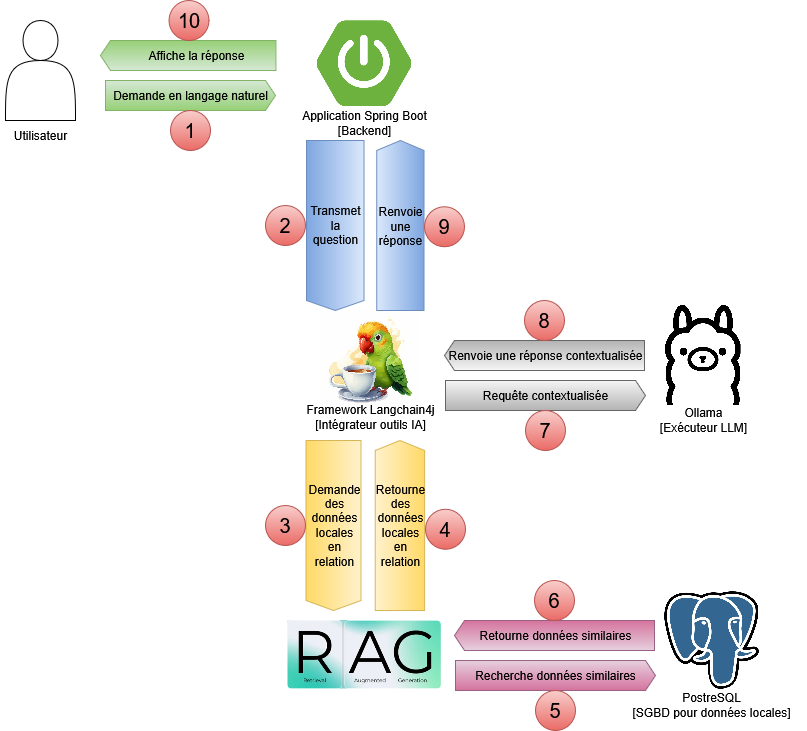
\includegraphics[width=1\textwidth]{illustration-graphique.drawio.png}
		\caption{Diagramme d'architecture}
		\label{fig:illustration-graphique}
	\end{figure}
	
	
	
	\section{Premier prototype}
	
	\subsection{Introduction}
	
	Pour atteindre cet objectif ambitieux, nous avons suivi une approche incrémentale. Dans un premier temps, un prototype fonctionnel a été réalisé afin de valider les fondements techniques du projet. Ce prototype est une application basée sur un agent intelligent exploitant une architecture RAG (Retrieval-Augmented Generation), capable de répondre aux questions de l’utilisateur à partir d’un document texte ou PDF fourni. Cette première version a permis de :
	\begin{itemize}
		\item comprendre le fonctionnement du framework LangChain4j ;
		\item tester l’intégration avec le LLM Ollama ;
		\item valider le concept de récupération de contexte à partir de documents externes.
	\end{itemize}
	
	\subsection{Fonctionnement d'un agent AI dans LangChain4j}
	
	Dans LangChain4j, un Agent AI orchestre les interactions entre un ChatLanguageModel (abstraction des LLMs comme OpenAI/Gemini/Ollama) et un ChatMemoryProvider (gestion de l'historique conversationnel). L'Agent formate les requêtes, intègre la mémoire contextuelle, et peut utiliser des outils externes, tandis que le LLM génère les réponses. Cette architecture modulaire permet une intégration flexible avec différents modèles et systèmes de stockage, tout en maintenant un état conversationnel cohérent.
	
	Le diagramme de séquences suivant décrit ce processus :
	
	\begin{figure}[H]
		\centering
		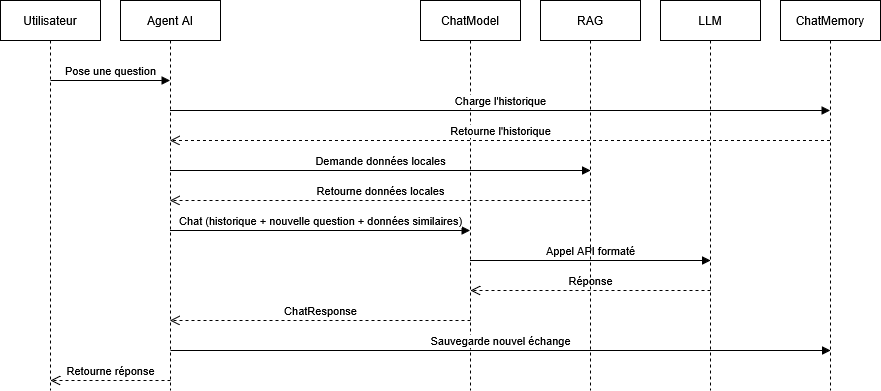
\includegraphics[width=\textwidth]{ds-ai-agent.drawio.png}
		\caption{Diagramme de séquences décrivant le fonctionnement d'un agent AI}
		\label{fig:ds-ai-agent.drawio}
	\end{figure}
	
	Le RAG combine deux phases clés pour améliorer la génération de réponses par un LLM : la rétroinformation (retrieval) et la génération contextuelle. Dans ce prototype, le système RAG :
	
	\begin{itemize}
		\item Charge d’abord un fichier source (texte, PDF, etc.).
		\item Utilise un DocumentPaser pour extraire les données brutes, et les découper en 'chunks'.
		\item Utilise un EmbeddingModel qui convertit ces chunks en vecteurs d’embedding (représentations numériques sémantiques).
		\item Utilise un EmbeddingStoreIngestor pour stocker ces vecteurs dans un EmbeddingStore.
		\item Utilise un Retriever qui interroge l’EmbeddingStore pour trouver les documents les plus pertinents par rapport à la question de l'utilisateur.
	\end{itemize}
	
	Le diagramme de séquences suivant détaille ces étapes :
	
	\begin{figure}[H]
		\centering
		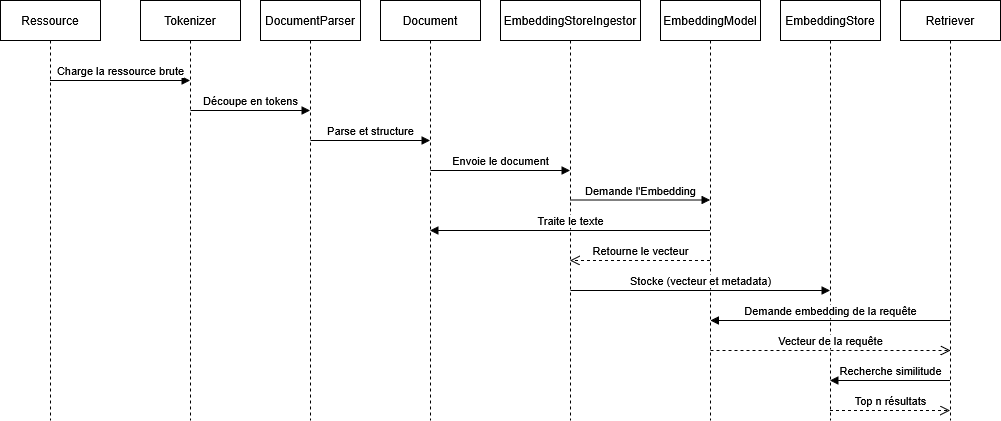
\includegraphics[width=\textwidth]{ds-rag.drawio.png}
		\caption{Diagramme de séquences décrivant le fonctionnement du RAG}
		\label{fig:ds-rag.drawio}
	\end{figure}
	
	Pour tester ce prototype, nous avons fourni un fichier PDF, son contenu est une lettre de recommandation pour une étudiante appelée Nour, on a ensuite envoyé une question à propos de cette étudiante à l'agent AI, en utilisant un contrôleur web :
	
	\begin{figure}[H]
		\centering
		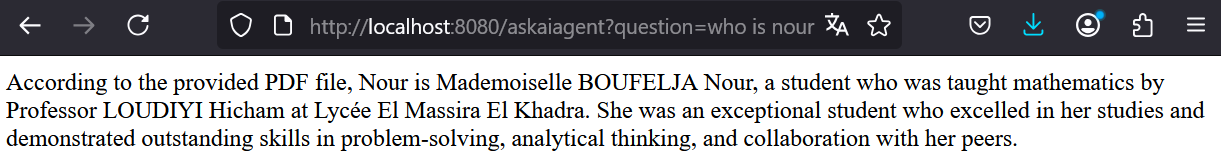
\includegraphics[width=\textwidth]{test-rag.png}
		\caption{Test du RAG}
		\label{fig:test-rag}
	\end{figure}
	
	
	
\end{document}}